\documentclass{beamer}

\usetheme{Boadilla}
% \usecolortheme{beaver} % --- We are replacing this with our own theme below ---

\usepackage{amsmath}
\usepackage{amssymb}
\usepackage{graphicx}
\usepackage{physics}
\usepackage{mathtools}
\usepackage{siunitx}
\usepackage{tikz}
\usetikzlibrary{positioning, shapes.geometric, arrows.meta}
\usepackage{booktabs}
\usepackage{lmodern}
\usepackage{setspace}
\onehalfspacing
\usepackage[bottom]{footmisc}

% --- CUSTOM COLOR THEME SETUP ---

% 1. Define your new colors using Hex codes
\definecolor{ULBBlue}{HTML}{0D47A1}
\definecolor{ULBTeal}{HTML}{4DB6AC}
\definecolor{VUBOrange}{HTML}{E87722}
\definecolor{AlertColor}{HTML}{D32F2F}
\definecolor{LightGray}{HTML}{F5F5F5}


% 2. Apply these colors to Beamer's elements
\setbeamercolor{palette primary}{bg=ULBBlue, fg=white}
\setbeamercolor{palette secondary}{bg=VUBOrange, fg=white}
\setbeamercolor{palette tertiary}{bg=ULBBlue, fg=white}
\setbeamercolor{palette quaternary}{bg=VUBOrange, fg=white}

\setbeamercolor{structure}{fg=ULBBlue} % This is a key color for many elements
\setbeamercolor{titlelike}{bg=ULBBlue, fg=white}
\setbeamercolor{frametitle}{bg=ULBBlue, fg=white}
\setbeamercolor{title}{use=structure,fg=white,bg=structure.fg}

\setbeamercolor{normal text}{fg=black, bg=white}
\setbeamercolor{block title}{use=structure,fg=white,bg=structure.fg}
\setbeamercolor{block body}{bg=LightGray}
\setbeamercolor{alerted text}{fg=AlertColor}

% --- END OF CUSTOM COLOR THEME ---

% --- Command to automatically create a title slide for each section ---
\AtBeginSection[]{
	\begin{frame}
		\vfill
		\centering
		\begin{beamercolorbox}[sep=8pt,center,shadow=true,rounded=true]{title}
			\usebeamerfont{title}\insertsectionhead\par%
		\end{beamercolorbox}
		\vfill
	\end{frame}
}
% --- END of command ---


\title[TDL Wideband and Narrowband Channel Models]{Question 1: TDL Wideband and Narrowband Channel Models}
\subtitle{Demonstration and Statistical Models for Taps in Wideband Case}
\author{Cédric Sipakam}
\institute{ULB | VUB \\
	\vspace{1.5em}
	ELEC-H415: Communication Channels}
\date{2025}


\setbeamertemplate{footline}
{
	\leavevmode%
	\hbox{%
		\begin{beamercolorbox}[wd=.5\paperwidth,ht=2.25ex,dp=1ex,left]{author in head/foot}%
			\hspace*{2ex}\usebeamerfont{title in head/foot}\insertshorttitle%
		\end{beamercolorbox}%
		\begin{beamercolorbox}[wd=.5\paperwidth,ht=2.25ex,dp=1ex,right]{title in head/foot}%
			\usebeamerfont{page number in head/foot}\insertframenumber{} / \inserttotalframenumber\hspace*{2ex}%
		\end{beamercolorbox}%
	}%
	\vskip0pt%
}



\begin{document}
	\begin{frame}
		\begin{figure}
			\centering
			
\includegraphics[width=0.7\linewidth]{pictures/logos}
		\end{figure}
		\titlepage
	\end{frame}
	
	\begin{frame}{Outline}
		\tableofcontents
	\end{frame}
	
	\section{Introduction}
	
	\begin{frame}{Wireless Communication Channel}
		\begin{itemize}
			\item A communication channel is the medium through which the electromagnetic signal propagates.
			\item It is characterized by three main phenomena:
			\begin{itemize}
				\item \textbf{Attenuation}: Reduction in signal strength over distance.
				\item \textbf{Time Dispersion}: Signal spreading over time due to multipath propagation.
				\item \textbf{Fading}: Fluctuations in signal amplitude and phase.
			\end{itemize}
		\end{itemize}
		\begin{figure}
			\centering
			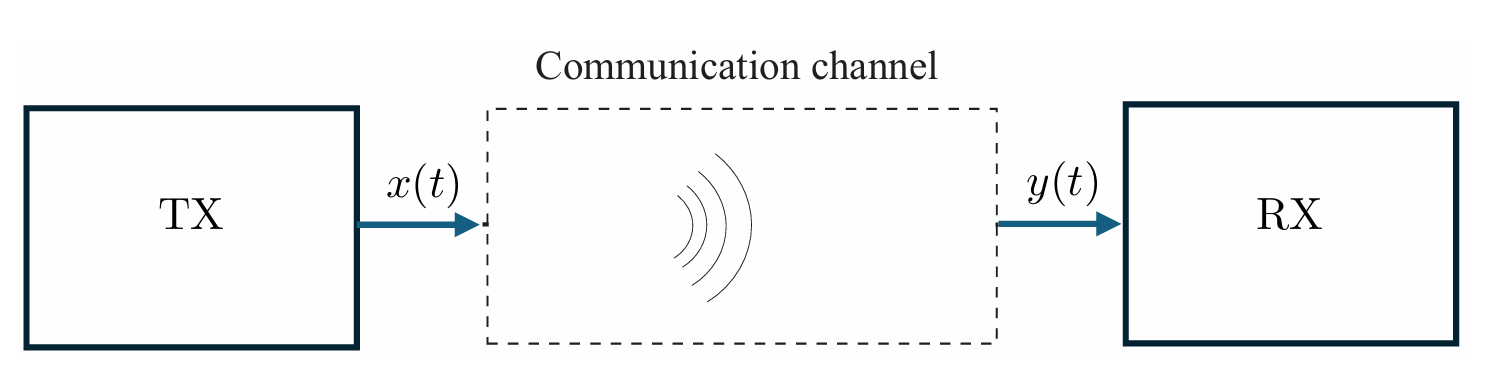
\includegraphics[width=0.8\linewidth]{"pictures/wireless-comm-channel.png"}
			\caption{Basic communication system diagram}
		\end{figure}
	\end{frame}
	
	
	\begin{frame}{Physical Impulse Response of the Channel}
		\begin{itemize}
			\item The physical channel is described by its time-varying impulse response, $h(\tau, t)$.
			\item It is a sum of delayed Dirac delta functions, each representing a multipath component (MPC):
			\[
			h(\tau,t) = \sum_{n=1}^{N} \alpha_n(t) \delta(\tau - \tau_n)
			\]
		\end{itemize}
	\end{frame}
	
	\begin{frame}{Physical Impulse Response of the Channel}
		\begin{itemize}
			\item The term $\alpha_n(t)$ is the complex amplitude of the $n$\textsuperscript{th} MPC:
			\[
			\alpha_n(t) = a_n(t) e^{j\phi_n(t)} e^{-j2\pi f_c \tau_n}
			\]
			\begin{itemize}
				\item $a_n(t)$: Real amplitude.
				\item $\phi_n(t)$: Phase shift.
				\item $\tau_n$: Propagation delay.
			\end{itemize}
		\end{itemize}
	\end{frame}
	
	\begin{frame}{Received Signal Formulation}
		\begin{itemize}
			\item The received baseband signal $y(t)$ is the convolution of the transmitted signal $x(t)$ with the channel's impulse response:
			\[
			y(t) = \int_0^{\infty} h(\tau, t) x(t - \tau) \, d\tau
			\]
			\item Substituting the physical impulse response gives:
			\[
			y(t) = \sum_{n=1}^{N} \alpha_n(t) x(t - \tau_n)
			\]
		\end{itemize}
	\end{frame}
	
	\begin{frame}{Received Signal Formulation}
		\begin{figure}
			\centering
			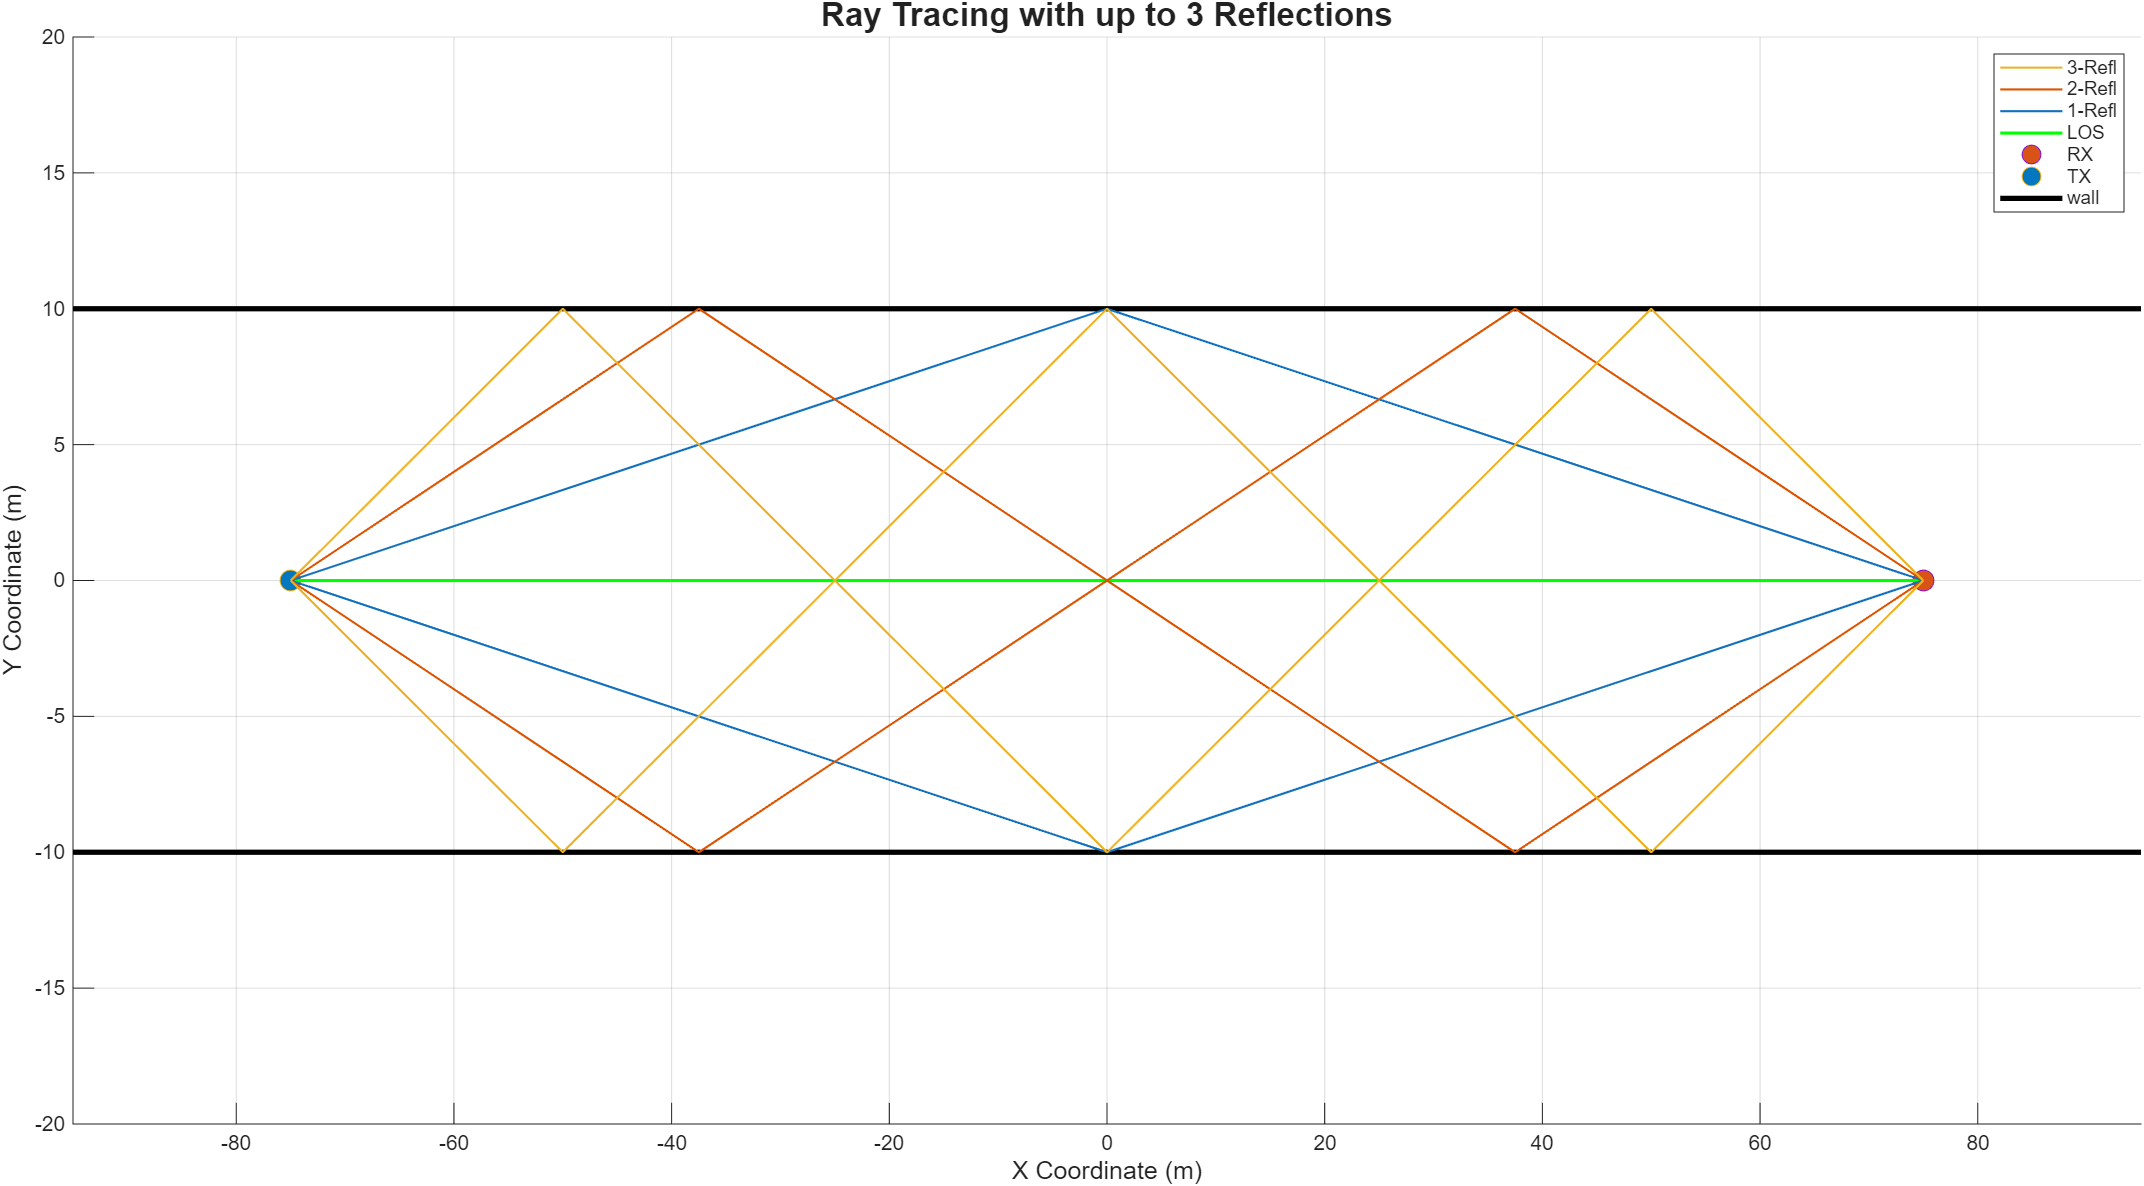
\includegraphics[width=0.9\linewidth]{"pictures/ray-tracing-3-reflections.png"}
			\caption{Diagram of multipath components arriving at the receiver.}
		\end{figure}
	\end{frame}
	
	
	\section{Tapped Delay Line Models}
	\begin{frame}{The Problem of Limited Bandwidth}
		\centering
		\resizebox{1\textwidth}{!}{
			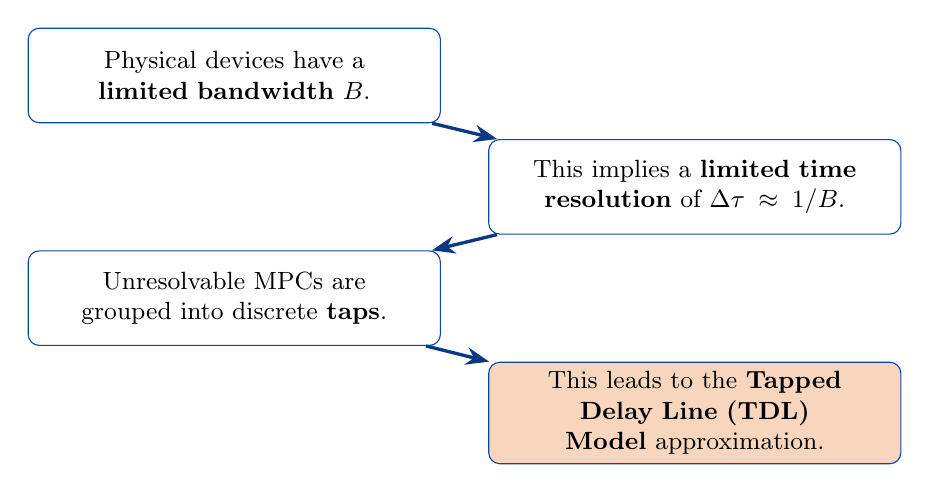
\begin{tikzpicture}[
				node distance=0.2cm and 0.6cm,
				mybox/.style={
					draw=ULBBlue,
					rectangle,
					rounded corners,
					text centered,
					text width=5cm,
					minimum height=1.2cm,
					font=\small
				},
				arrow/.style={
					->,
					very thick,
					>=Stealth,
					draw=ULBBlue!80!black
				}
				]
				\node[mybox] (bw) {Physical devices have a \textbf{limited bandwidth} $B$.};
				\node[mybox, below right=of bw] (res) {This implies a \textbf{limited time resolution} of $\Delta\tau \approx 1/B$.};
				\node[mybox, below left=of res] (mpc) {Unresolvable MPCs are grouped into discrete \textbf{taps}.};
				\node[mybox, below right=of mpc, fill=VUBOrange!30, text=black] (tdl) {This leads to the \textbf{Tapped Delay Line (TDL) Model} approximation.};
				\draw[arrow] (bw) -- (res);
				\draw[arrow] (res) -- (mpc);
				\draw[arrow] (mpc) -- (tdl);
			\end{tikzpicture}
		}
	\end{frame}
	
	\section{Narrowband TDL Model}
	
	\begin{frame}{Condition for Narrowband}
		\begin{itemize}
			\item Define the delay spread: $\sigma_\tau = \max_{i,j} |\tau_i - \tau_j|$
			\item And the coherence bandwidth: $\Delta f_c \approx \frac{1}{\sigma_\tau}$
		\end{itemize}
		\vspace{1em}
		A channel is \textbf{narrowband} if the signal bandwidth $B \ll \Delta f_c$, which implies:
		\[ \Delta\tau \gg \sigma_\tau \]
		
		\begin{block}{Consequence}
			All multipath components arrive within the same time resolution interval, $\Delta\tau$. They are therefore indistinguishable and combine into a single tap.
		\end{block}
	\end{frame}
	
	\begin{frame}{Condition for Narrowband}
		\begin{figure}
			\centering
			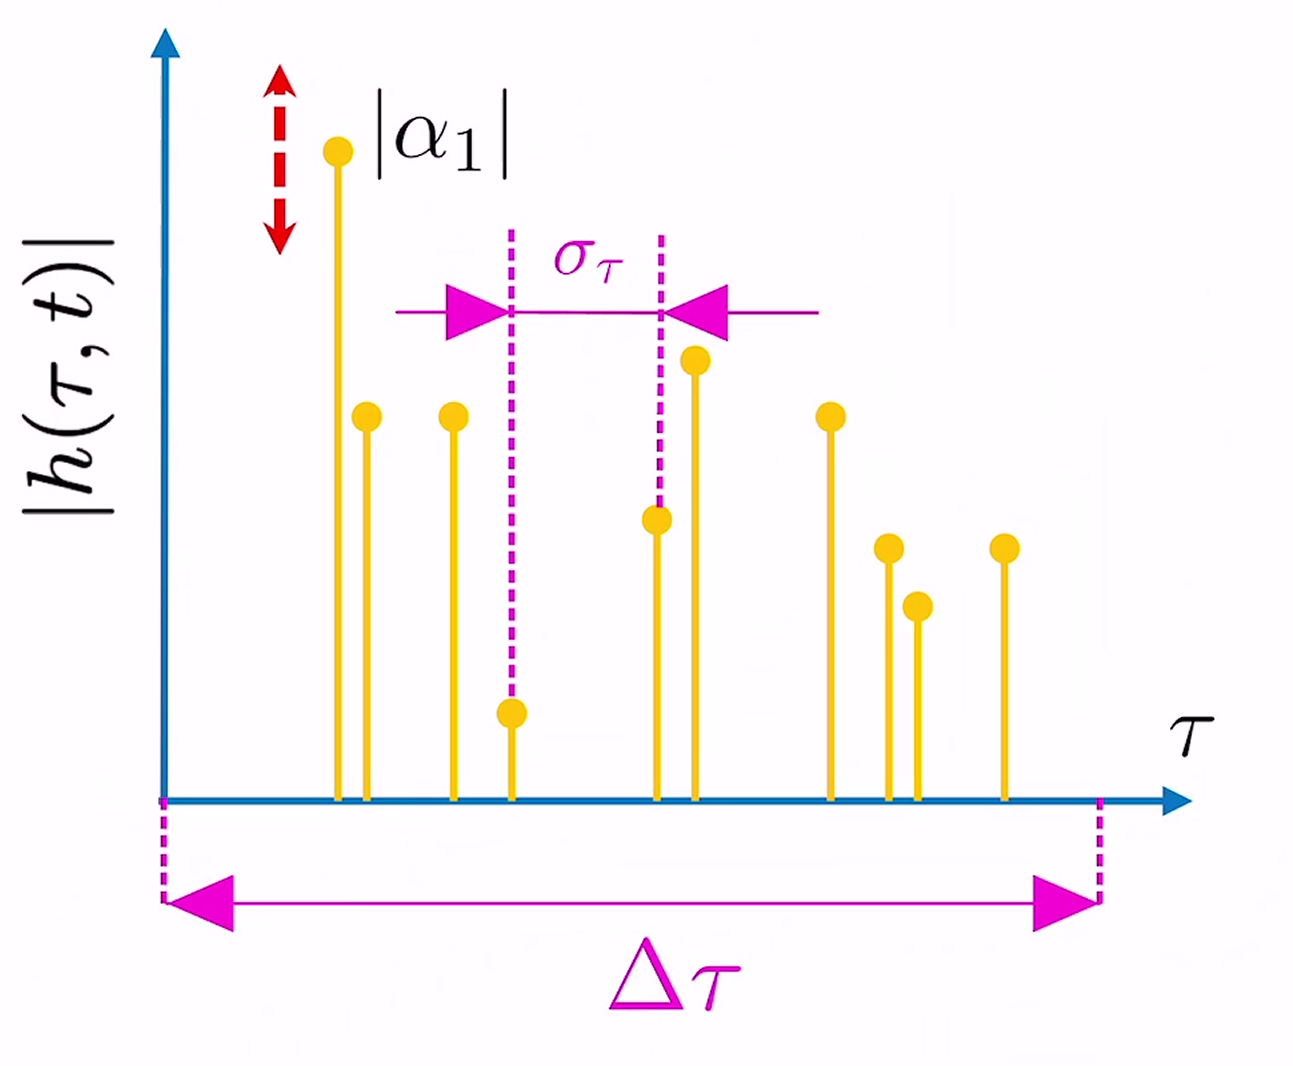
\includegraphics[width=0.6\linewidth]{pictures/narrowband-condition}
			\caption{Diagram showing a large $\Delta\tau$ encompassing all MPCs.}
		\end{figure}
	\end{frame}
	
	\begin{frame}{Derivation of the Narrowband Model}
		\begin{itemize}
			\item Since all MPCs are unresolvable, the TDL model simplifies to a single tap at $\tau=0$:
			\[ h_{TDL}(\tau, t) = h_0(t) \delta(\tau) \]
			
			\item The coefficient $h_0(t)$, or simply $h(t)$, is the coherent sum of all multipath components:
			\[ h(t) \approx \sum_{n=1}^{N} \alpha_n(t) = \sum_{n=1}^{N} a_n(t) e^{j\phi_n(t)} e^{-j2\pi f_c \tau_n} \]
		\end{itemize}
	\end{frame}
	
	\begin{frame}{Derivation of the Narrowband Model}
		\begin{itemize}
			\item The received signal becomes a simple product:
			\[ y(t) = \int_0^{\infty} h(t)\delta(\tau) x(t - \tau) \, d\tau = h(t)x(t) \]
			
			\item The channel transfer function $H(f,t)$ is independent of the baseband frequency $f$:
			\[ H(f,t) = \int_{-\infty}^{\infty} h(t)\delta(\tau) e^{-j2\pi f \tau} \, d\tau = h(t) \]
			This is known as \textbf{flat fading}.
		\end{itemize}
	\end{frame}
	
	\section{Wideband TDL Model}
	
	\begin{frame}{Condition for Wideband}
		A channel is \textbf{wideband} when the signal bandwidth $B$ is comparable to or larger than the coherence bandwidth $\Delta f_c$, which implies the time resolution $\Delta\tau$ is smaller than the delay spread $\sigma_\tau$.
		\[ \Delta\tau < \sigma_\tau \]
		
		\begin{block}{Consequence}
			The system's time resolution is fine enough to resolve groups of multipath components. This leads to a model with multiple taps, causing frequency-selective fading.
		\end{block}
	\end{frame}
	
	\begin{frame}{Condition for Wideband}
		\begin{figure}
			\centering
			\includegraphics[width=0.6\linewidth]{pictures/wideband-condition"}
			\caption{Diagram showing a small $\Delta\tau$ resolving different MPCs.}
		\end{figure}	
	\end{frame}
	
	\begin{frame}{Derivation of the Wideband Model (1/2)}
		\begin{itemize}
			\item The bandlimited signal $x(t)$ allows us to use the sampling theorem. The delayed signal $x(t-\tau)$ can be written as:
			\[ x(t-\tau) = \sum_{l=-\infty}^{\infty} x(t-l\Delta\tau) \text{sinc}(B(\tau - l\Delta\tau)) \]
			
			\item We substitute this into the convolution integral for $y(t)$:
			\[ y(t) = \int_0^{\infty} h(\tau, t) \sum_{l} x(t-l\Delta\tau) \text{sinc}(B(\tau-l\Delta\tau)) d\tau \]
		\end{itemize}
	\end{frame}
	
	\begin{frame}{Derivation of the Wideband Model (2/2)}
		\begin{itemize}
			\item Swapping the integral and summation:
			\[ y(t) = \sum_{l} x(t-l\Delta\tau) \underbrace{\int_0^{\infty} h(\tau, t) \text{sinc}(B(\tau-l\Delta\tau)) d\tau}_{\equiv h_l(t)} \]
			
			\item This gives the discrete-time convolution model:
			\[ y(t) = \sum_{l=0}^{L} h_l(t) x(t-l\Delta\tau) \]
		\end{itemize}
	\end{frame}
	
	\begin{frame}{The Taps of the Wideband Model}
		\begin{itemize}
			\item The resulting impulse response is the Tapped Delay Line (TDL) model:
			\[ h_{TDL}(\tau, t) = \sum_{l=0}^{L} h_l(t) \delta(\tau - l\Delta\tau) \]
			
			\item Substituting the physical model for $h(\tau,t)$, the exact tap gain is:
			\[ h_l(t) = \sum_{n=1}^{N} \alpha_n(t) \text{sinc}(B(\tau_n - l\Delta\tau)) \]
			
			\item This can be approximated as the sum of all MPCs whose delays $\tau_n$ fall within the $l$-th time bin:
			\[ h_l(t) \approx \sum_{\tau_n \, \in \, \text{tap l}} \alpha_n(t) \]
		\end{itemize}
	\end{frame}
	
	\begin{frame}{Visualizing the Taps}
		\begin{block}{Consequence}
			Each tap represents the interference of all MPCs arriving around the delay $l\Delta\tau$. The physical, continuous impulse response is sampled into a discrete TDL model.
		\end{block}
	\end{frame}
	
	\begin{frame}{Visualizing the Taps}
		\begin{figure}
			\centering
			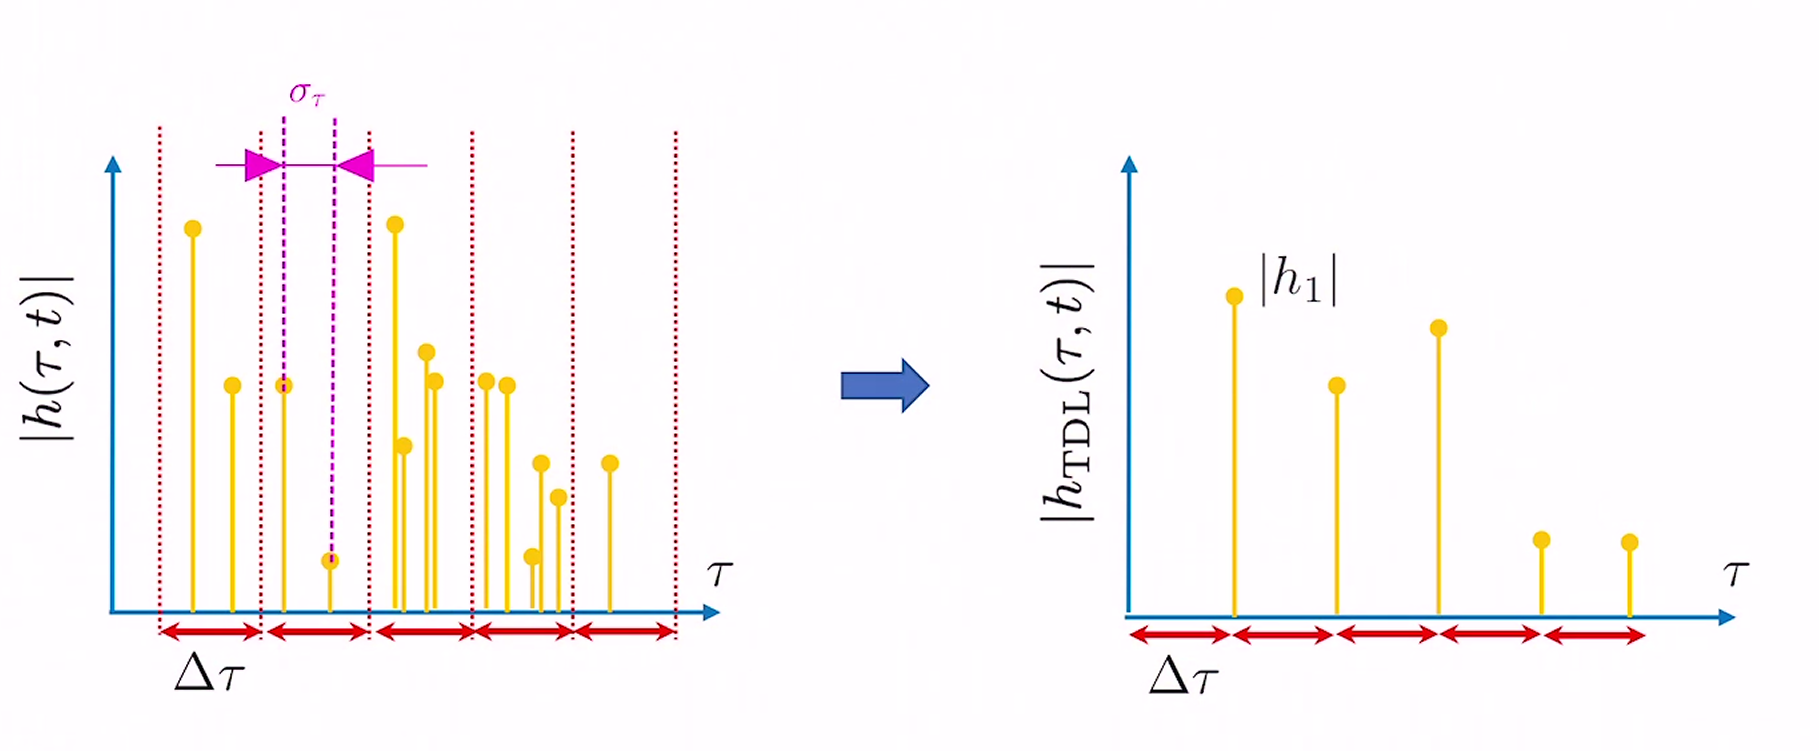
\includegraphics[width=0.9\linewidth]{pictures/tdl-grouping.png}
			\caption{Grouping of physical MPCs into discrete taps.}
		\end{figure}
	\end{frame}
	
	\section{Wideband Scenario - Statistical Model}
	
	\begin{frame}{Motivation for a Statistical Approach}
		\begin{itemize}
			\item A deterministic model (like ray-tracing) is often impractical. The exact properties of each MPC are highly sensitive to small changes in the environment.
			\item A statistical model aims to generate a channel with the same statistical properties (e.g., average power, fading distribution) as a real channel.
		\end{itemize}
	\end{frame}
	
	\begin{frame}{Motivation for a Statistical Approach}
		\begin{itemize}
			\item We model the complex tap coefficients $h_l(t)$ as random variables.
			\item The phases $\Phi_n$ of the constituent MPCs are assumed to be independent and uniformly distributed in $[0, 2\pi)$.
			\[ h_l(t) = \sum_{\tau_n \in \text{tap } l} a_n e^{j\Phi_n} \]
		\end{itemize}
	\end{frame}
	
	\begin{frame}{Rayleigh Fading Taps (NLOS)}
		\begin{itemize}
			\item \textbf{Hypothesis}: A tap consists of a large number of MPCs, with no single component being significantly stronger than the others (Non-Line-of-Sight condition).
			
			\item By the \textbf{Central Limit Theorem}, $h_l(t)$ converges to a complex Gaussian random variable with zero mean.
			\[ h_l(t) = X_l + jY_l \quad \text{where } X_l, Y_l \sim \mathcal{N}(0, \sigma_l^2) \]
			
			\item The envelope, $|h_l(t)| = \sqrt{X_l^2 + Y_l^2}$, follows a \textbf{Rayleigh distribution}.
		\end{itemize}
	\end{frame}
	
	\begin{frame}{The Rayleigh Distribution}
		\begin{itemize}
			\item Probability Density Function (PDF):
			\[ p(|h_l|) = \frac{|h_l|}{\sigma_l^2} \exp\left(-\frac{|h_l|^2}{2\sigma_l^2}\right) \]
			
			\item Cumulative Distribution Function (CDF):
			\[ F(|h_l|) = \int_0^{|h_l|} p(x) dx = 1 - \exp\left(-\frac{|h_l|^2}{2\sigma_l^2}\right) \]
			
			\item Expected values:
			\[ \mathbb{E}[|h_l|] = \sigma_l \sqrt{\frac{\pi}{2}}, \quad \mathbb{E}[|h_l|^2] = 2\sigma_l^2 \]
		\end{itemize}
	\end{frame}
	
	\begin{frame}{The Rayleigh Distribution}
		\begin{figure}
			\centering
			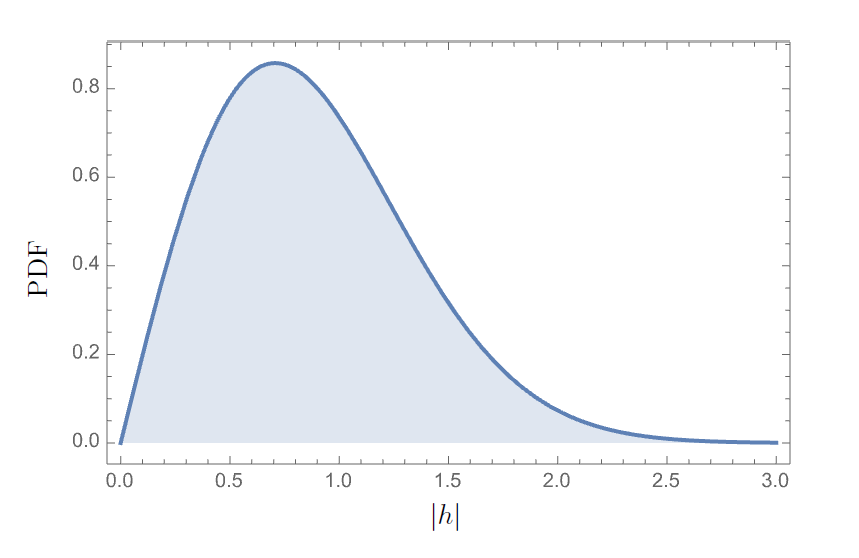
\includegraphics[width=0.7\linewidth]{"pictures/rayleigh-pdf.png"}
			\caption{Plot of the Rayleigh PDF.}
		\end{figure}
	\end{frame}
	
	\begin{frame}{Rician Fading Taps (LOS)}
		\begin{itemize}
			\item \textbf{Hypothesis}: A tap contains a dominant, stable component (typically a Line-of-Sight path), plus many weaker, scattered components.
			\[ h_l(t) = \underbrace{A_l e^{j\theta_l}}_{\text{Dominant}} + \underbrace{\sum a_n e^{j\Phi_n}}_{\text{Scattered}} \]
			
			\item The tap coefficient $h_l(t)$ is a complex Gaussian variable with a \textbf{non-zero mean}.
			
			\item The envelope $|h_l(t)|$ follows a \textbf{Rician distribution}.
		\end{itemize}
	\end{frame}
	
	\begin{frame}{The Rician Distribution}
		\begin{itemize}
			\item The PDF is given by:
			\[ p(|h_l|) = \frac{|h_l|}{\sigma_l^2} \exp\left(-\frac{|h_l|^2 + A_l^2}{2\sigma_l^2}\right) I_0\left(\frac{|h_l|A_l}{\sigma_l^2}\right) \]
			
			\item It is characterized by the \textbf{Rician K-factor}, the ratio of dominant to scattered power:
			\[ K_l = \frac{A_l^2}{2\sigma_l^2} \]
		\end{itemize}
	\end{frame}
	
	\begin{frame}{The Rician Distribution}
		\begin{figure}
			\centering
			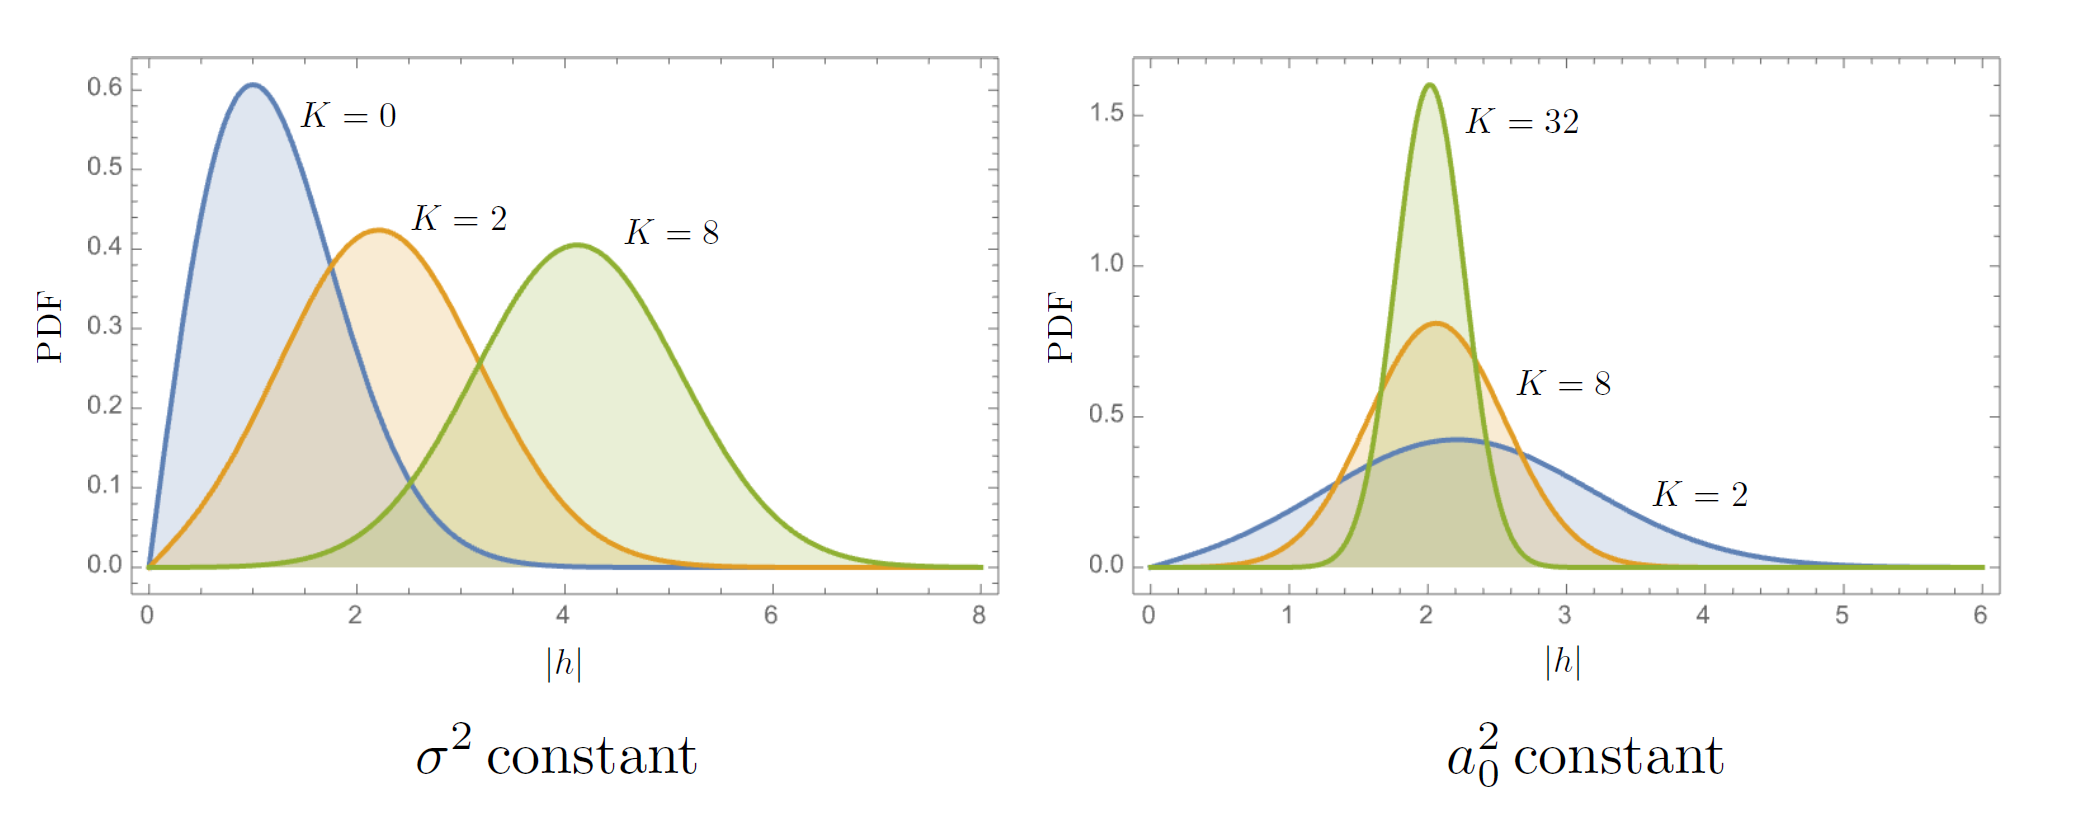
\includegraphics[width=\linewidth]{pictures/rician-pdf.png}
			\caption{Plot of Rician PDFs for different K-factors.}
		\end{figure}
	\end{frame}
	
	
	
	\begin{frame}{Example: Standardized PDP}
		\begin{block}{ITU Vehicular A model}
			A standard model for vehicle communications in an urban environment.
			\begin{center}
				\begin{tabular}{ccc}
					\toprule
					Tap & Delay [ns] & Avg. Power [dB] \\
					\midrule
					1 & 0 & 0 \\
					2 & 310 & -1.0 \\
					3 & 710 & -9.0 \\
					4 & 1090 & -10.0 \\
					5 & 1730 & -15.0 \\
					6 & 2510 & -20.0 \\
					\bottomrule
				\end{tabular}
			\end{center}
			All taps in this specific model are defined as having Rayleigh fading.
		\end{block}
	\end{frame}
	
	\section{Conclusion}
	
	\begin{frame}{Summary of Models}
		\begin{block}{Narrowband Model}
			\begin{itemize}
				\item Condition: $\Delta\tau \gg \sigma_\tau$
				\item Model: $y(t) = h(t)x(t)$
				\item Physical Effect: Flat fading
			\end{itemize}
		\end{block}
		
		\begin{block}{Wideband Model}
			\begin{itemize}
				\item Condition: $\Delta\tau < \sigma_\tau$
				\item Model: $y(t) = \sum h_l(t)x(t-l\Delta\tau)$
				\item Physical Effect: Frequency-selective fading
			\end{itemize}
		\end{block}
	\end{frame}
	
	\begin{frame}{Final Conclusion}
		\begin{alertblock}{Statistical Modeling of Taps}
			The complex nature of multipath propagation makes a statistical approach essential for wideband channels. By modeling taps as Rayleigh (NLOS) or Rician (LOS) random processes, parameterized by a standard Power Delay Profile, we can accurately simulate the behavior of real-world frequency-selective channels for system design and performance analysis.
		\end{alertblock}
	\end{frame}
	
\end{document}
